\chapter{Descripción del sistema}
\label{cap:capitulo5}

%La automatización de tareas agrícolas mediante tecnologías de visión artificial es una línea de investigación en plena expansión, especialmente en lo que respecta a la cosecha de productos delicados como las frutas, y más concretamente, las fresas. La maduración irregular, la variabilidad del entorno y la necesidad de recolección selectiva representan retos importantes, por lo que este proyecto nace con el propósito de aportar una solución basada en visión artificial y robótica colaborativa que permita mejorar la eficiencia y precisión en la recolección, reduciendo la intervención humana y el riesgo de daños al fruto.\\

%El presente Trabajo de Fin de Grado se enmarca en el desarrollo de un sistema de visión por ordenador para la detección de fresas maduras, con el objetivo de facilitar su recolección mediante un brazo robótico de la marca Universal Robots (UR). Este sistema propuesto permite detectar visualmente las fresas y estimar su posición en el espacio tridimensional utilizando una única cámara, integrando los datos en tiempo real con el robot colaborativo para ejecutar tareas de recolección automática.

Una vez expuestos el contexto, el estado del arte, los objetivos del proyecto y las plataformas de desarrollo empleadas, en este capítulo se describe de forma detallada el prototipo desarrollado (Figura \ref{fig:montaje_final}), y se abordan tanto los fundamentos teóricos que lo sustentan como el proceso seguido para su diseño e implementación, con el objetivo de ofrecer una visión completa del funcionamiento del sistema.

\begin{figure} [H]
    \begin{center}
      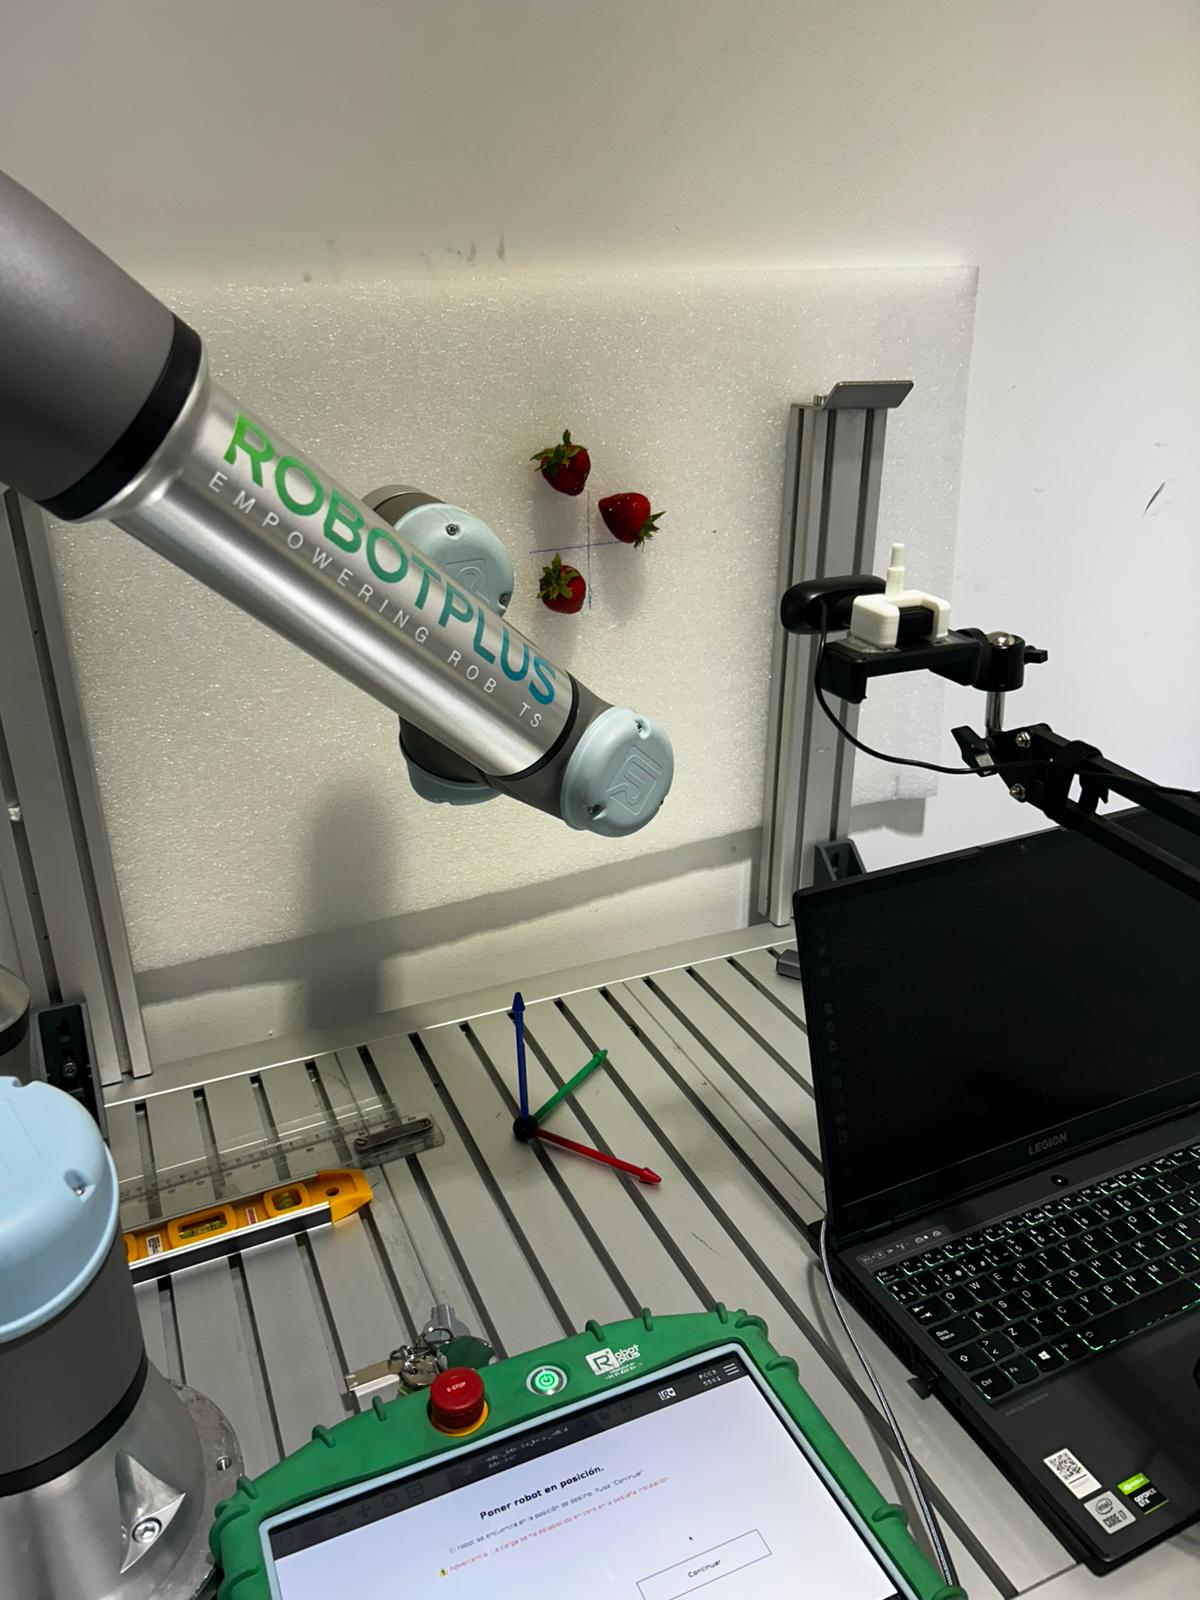
\includegraphics[width=9cm]{figs/Pruebas plano vertical deteccion multiple_editada.jpeg}
    \end{center}
    \caption{Montaje del sistema final con un UR5e}
    \label{fig:montaje_final}
\end{figure}
  

\section{Hipótesis suelo adaptada al plano vertical}
\label{sec:HS_vertical}

En el sistema propuesto, la estimación de coordenadas tridimensionales de las fresas a recolectar se basa en la hipótesis suelo, y se realiza a partir de una única cámara estenopeica RGB fija para poder realizar esta estimación sin recurrir a sensores adicionales. Esta técnica de simplificación empleada en visión por ordenador asume que los objetos de interés se encuentran sobre un plano conocido y fijo respecto a la cámara.

La hipótesis suelo (\cite{Vega21}, Figura \ref{fig:HS}) supone que todos los objetos del mundo en 3D están apoyados sobre el suelo, por lo tanto, asumiendo que el suelo está en el plano Z = 0, nos permitirá estimar, con el uso de la cámara, la posición 3D de los puntos que estén en el suelo.

\begin{figure} [H]
    \begin{center}
      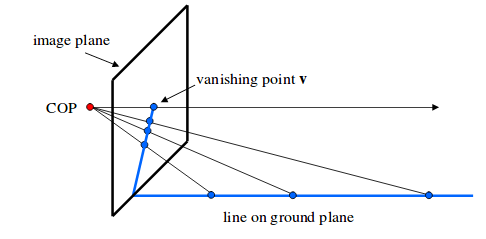
\includegraphics[width=9cm]{figs/Hipotesis suelo.png}
    \end{center}
    \caption{La hipótesis suelo asume que todos los objetos están en el suelo}
    \label{fig:HS}
\end{figure}

El hecho de que la cámara siga el modelo \textit{pinhole} o estenopeico, implica que la proyección de un punto en el espacio bidimensional de una imagen al tridimensional se realiza usando los parámetros intrínsecos de la propia cámara y parámetros extrínsecos como la rotación o la traslación de la misma (Cuadro \ref{tab:parametros_camara}). Al asumir que los puntos están sobre el plano Z=0 mediante la hipótesis suelo, este modelo estenopeico permite estimar las coordenadas X e Y reales a partir de la imagen captada por la cámara mediante una serie de fórmulas matemáticas (Ecuación \ref{ec:formulas_pinhole}).

 \begin{table}[H]
    \centering
    \begin{tabular}{cl}
      \toprule
      \textbf{Parámetros de cámara} & \textbf{Definición} \\
      \midrule
       K (3 × 3)   & Parámetros intrínsecos \\
       R (3 × 3)   & Rotación de la cámara \\
       T (3 × 1)   & Traslación de la cámara \\
      \bottomrule
    \end{tabular}
    \caption{Definición de los parámetros de posición y orientación de la cámara pinhole}
    \label{tab:parametros_camara}
  \end{table}
  
  \begin{myequation}[H]
    \begin{align} 
       w \cdot \begin{bmatrix} u \\ v \\ 1 \end{bmatrix}
       =
       K \cdot [R \,| \, T] \cdot \begin{bmatrix} X \\ Y \\ Z \\ 1 
    \end{bmatrix}
    \nonumber
    \end{align}
    \caption{Relación de fórmulas del modelo de cámara estenopeico}
    \label{ec:formulas_pinhole}
  \end{myequation}

En esta ecuación se observa la relación entre un punto tridimensional \((X, Y, Z)\) y su proyección bidimensional \((u, v)\) multiplicada por un factor de escala \(w\) que representa la profundidad del punto proyectado en la imagen captada por la cámara, donde la matriz de parámetros intrínsecos K (Ecuación \ref{ec:matriz_intrinsecos}) junto con las matrices de rotación R (Ecuación \ref{ec:rotacion_ejes}) y la matriz de traslación T de la cámara (Ecuación \ref{ec:matriz_traslacion}), constituyen la matriz de proyección. Esta matriz de proyección transforma los puntos tridimensionales al plano imagen. 

  \begin{myequation}[H]
    \begin{align}
      K = 
      \begin{pmatrix}
        F_x & 0   & C_x \\
        0   & F_y & C_y \\
        0   & 0   & 1
      \end{pmatrix}
      \nonumber
    \end{align}
    \caption{Matriz de parámetros intrínsecos de la cámara}
    \label{ec:matriz_intrinsecos}
  \end{myequation}

  \begin{myequation}[H]
    \begin{align*}
      R(\theta)_X &= 
      \begin{pmatrix}
        1 & 0 & 0 \\
        0 & \cos(\theta) & \sin(\theta) \\
        0 & -\sin(\theta) & \cos(\theta)
      \end{pmatrix} \\[2ex]
      \nonumber
      R(\theta)_Y &= 
      \begin{pmatrix}
        \cos(\theta) & 0 & -\sin(\theta) \\
        0 & 1 & 0 \\
        \sin(\theta) & 0 & \cos(\theta)
      \end{pmatrix} \\[2ex]
      \nonumber
      R(\theta)_Z &= 
      \begin{pmatrix}
        \cos(\theta) & -\sin(\theta) & 0 \\
        \sin(\theta) & \cos(\theta) & 0 \\
        0 & 0 & 1
        \nonumber
      \end{pmatrix}
    \end{align*}
    \caption{Matrices de rotación \( R(\theta) \) según el eje de rotación}
    \label{ec:rotacion_ejes}
  \end{myequation}


  \begin{myequation}[H]
    \begin{align}
      T =
      \begin{pmatrix}
        t_x \\
        t_y \\
        t_z
      \end{pmatrix}
    \nonumber
    \end{align}
    \caption{Matriz de traslación de la cámara en coordenadas tridimensionales}
    \label{ec:matriz_traslacion}
  \end{myequation}


Para poder obtener la proyección tridimensional a partir de la bidimensional habría que operar en la Ecuación \ref{ec:formulas_pinhole} para despejar las incógnitas \((X, Y, Z)\), siendo la distancia a la cámara constante y conocida (\( Z = Z_0) \) debido a la hipótesis suelo (Ecuación \ref{ec:inversion_pinhole}), ya que que se dispone de los parámetros intrínsecos de la cámara y la geometría del plano.

  \begin{myequation}[H]
    \begin{align*}
      &K^{-1} \cdot w \cdot 
      \begin{bmatrix}
        u \\
        v \\
        1
      \end{bmatrix}
      =
      R \cdot 
      \begin{bmatrix}
        X \\
        Y \\
        Z_0
      \end{bmatrix}
      + T \\[2ex]
      &\begin{bmatrix}
        X \\
        Y \\
        Z_0
      \end{bmatrix}
      =
      R^{-1} \cdot 
      \left(
      K^{-1} \cdot w \cdot 
      \begin{bmatrix}
        u \\
        v \\
        1
      \end{bmatrix}
      - T
      \right)
    \end{align*}
    \caption{Descomposición e inversión parcial del modelo de cámara pinhole para estimar las coordenadas tridimensionales de un punto conocido en imagen bajo la hipótesis suelo \(Z = Z_0\).}
    \label{ec:inversion_pinhole}
  \end{myequation}

En este caso, y debido a la orientación del escenario, la hipótesis suelo ha sido adaptada al plano vertical, lo que significa que se asume que las fresas están dispuestas sobre una superficie vertical conocida, como es el caso en los huertos verticales. En este plano de trabajo vertical, se ha establecido un sistema de coordenadas 3D, cuyo origen coincide con el punto central del campo de visión de la cámara, actuando como referencia para crear el plano de trabajo en el robot a través de su interfaz y utilizando las mismas orientaciones de los ejes de coordenadas de la cámara (Figura \ref{fig:Plano_pared_UR}). Esto permite que una vez realizado el cálculo de las coordenadas de las fresas detectadas y el de las distancias a cada detección (Ecuación \ref{ec:formula_distancia}), estas coincidan con las coordenadas en este plano vertical, simplificando de esta manera el proceso de transformación de las mismas. 

\begin{myequation}[H]
  \begin{align}
    \text{distancia} = \sqrt{X^2 + Y^2 + Z^2}
  \nonumber
  \end{align}
\caption{Fórmula del cálculo de la distancia de la cámara a las detecciones}
\label{ec:formula_distancia}
\end{myequation}


\begin{figure} [H]
    \begin{center}
      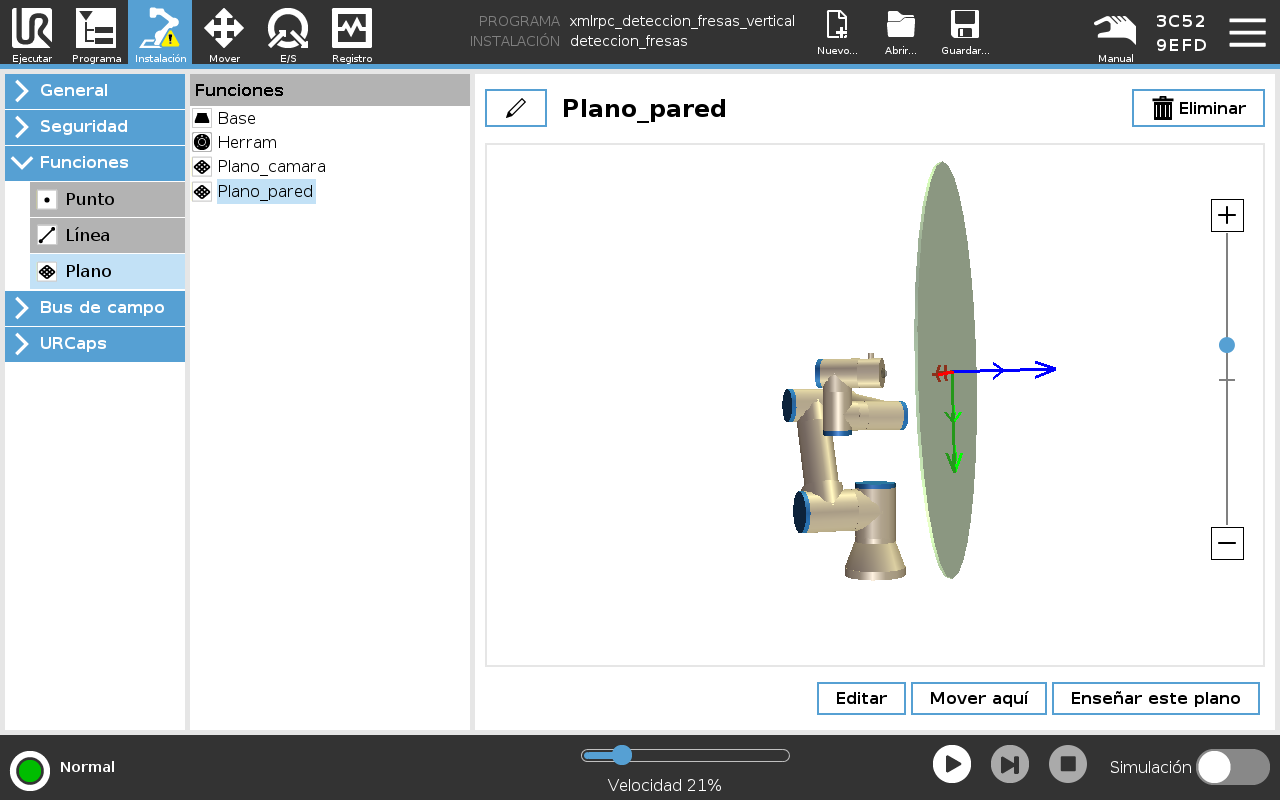
\includegraphics[width=155mm]{figs/Plano Pared Programa UR.png}
    \end{center}
    \caption{Plano pared generado en el UR}
    \label{fig:Plano_pared_UR}
\end{figure}


\section{Detección de fresas mediante Deep Learning}
\label{sec:Tecnica_Vision}

La detección de las fresas maduras se ha resuelto mediante el uso de técnicas de visión artificial basadas en deep learning, concretamente, se ha utilizado el modelo YOLOv3 (You Only Look Once), un detector de objetos en tiempo real ampliamente utilizado por su equilibrio entre precisión y velocidad, tal y como se define en la Sección \ref{sec:YOLOv3}.

Este modelo ha sido entrenado específicamente para reconocer fresas maduras en las condiciones del entorno de trabajo y, una vez entrenado, se ha integrado en un script que analiza el flujo de vídeo en tiempo real y devuelve las coordenadas y la distancia a la cámara de cada fresa detectada en la imagen, junto con la clase del objeto y la confianza de detección (Figura \ref{fig:deteccion_dl}).

\pagebreak
Para mejorar la precisión a la hora de estimar la posición de la fresa, se ha utilizado el centro del \textit{bounding box} de la fresa detectada como punto de referencia para la proyección sobre el plano vertical, conforme a la hipótesis descrita en la Sección \ref{sec:HS_vertical}.

\begin{figure} [H]
    \begin{center}
    \subcapcentertrue
    \subfigure[Ventana donde se muestran las detecciones\label{fig:ventana_deteccion}]{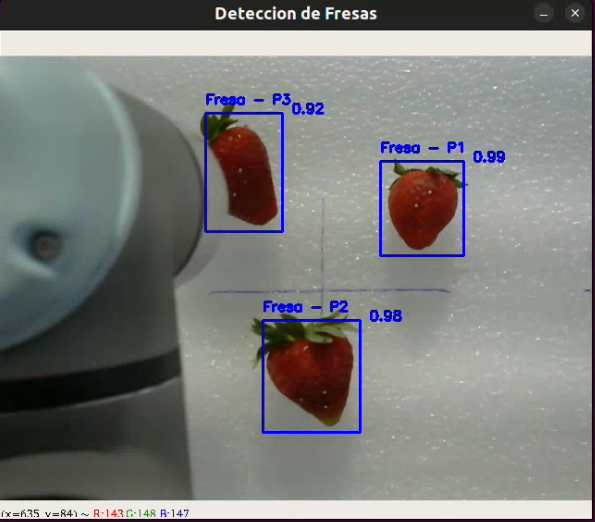
\includegraphics[width=9cm]{figs/POV Camara Pruebas plano vertical deteccion multiple UR5e_VENTANA.png}}
    \subfigure[Mensajes mostrados por la terminal al ejecutar el programa de detección\label{fig:mensajes_terminal}]{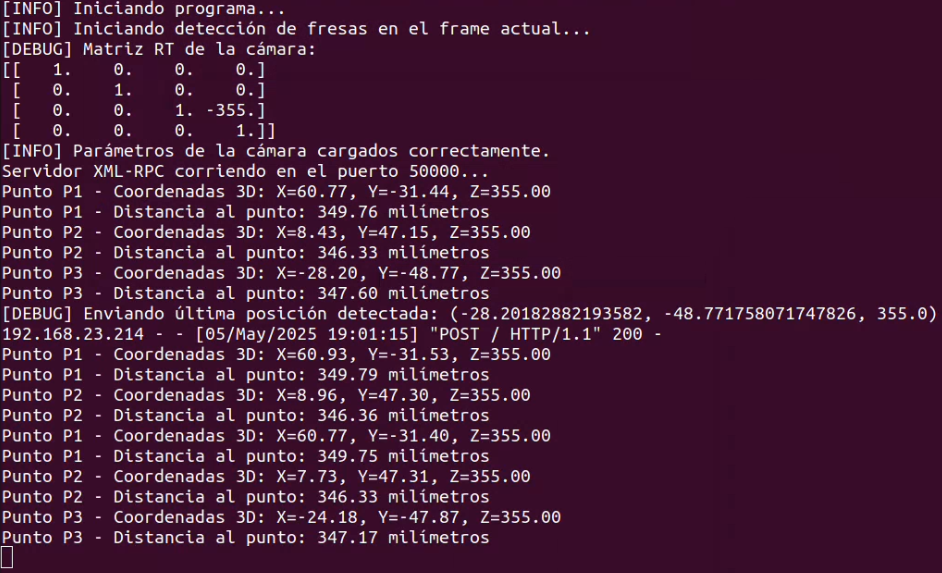
\includegraphics[width=14cm]{figs/POV Camara Pruebas plano vertical deteccion multiple UR5e_TERMINAL.png}}
    \end{center}
    \caption{Detección de fresas maduras mediante deep learning}
    \label{fig:deteccion_dl}
\end{figure}

\section{Arquitectura del sistema}
\label{sec:arquitectura_sistema}

El prototipo final se ha implementado utilizando una combinación de componentes hardware y software, descritos con detalle en el Capítulo \ref{cap:capitulo4}, específicamente seleccionados y configurados para responder a los requisitos del sistema de recolección automatizada. Esta integración ha sido diseñada para garantizar la detección precisa de fresas, el cálculo de su localización espacial en coordenadas tridimensionales y la ejecución del movimiento del robot sobre estas posiciones (Figura \ref{fig:UR5e_planopared}). 

  \begin{figure}[H]
      \begin{center}
        \subcapcentertrue
        \subfigure[Detección simple en el plano vertical]{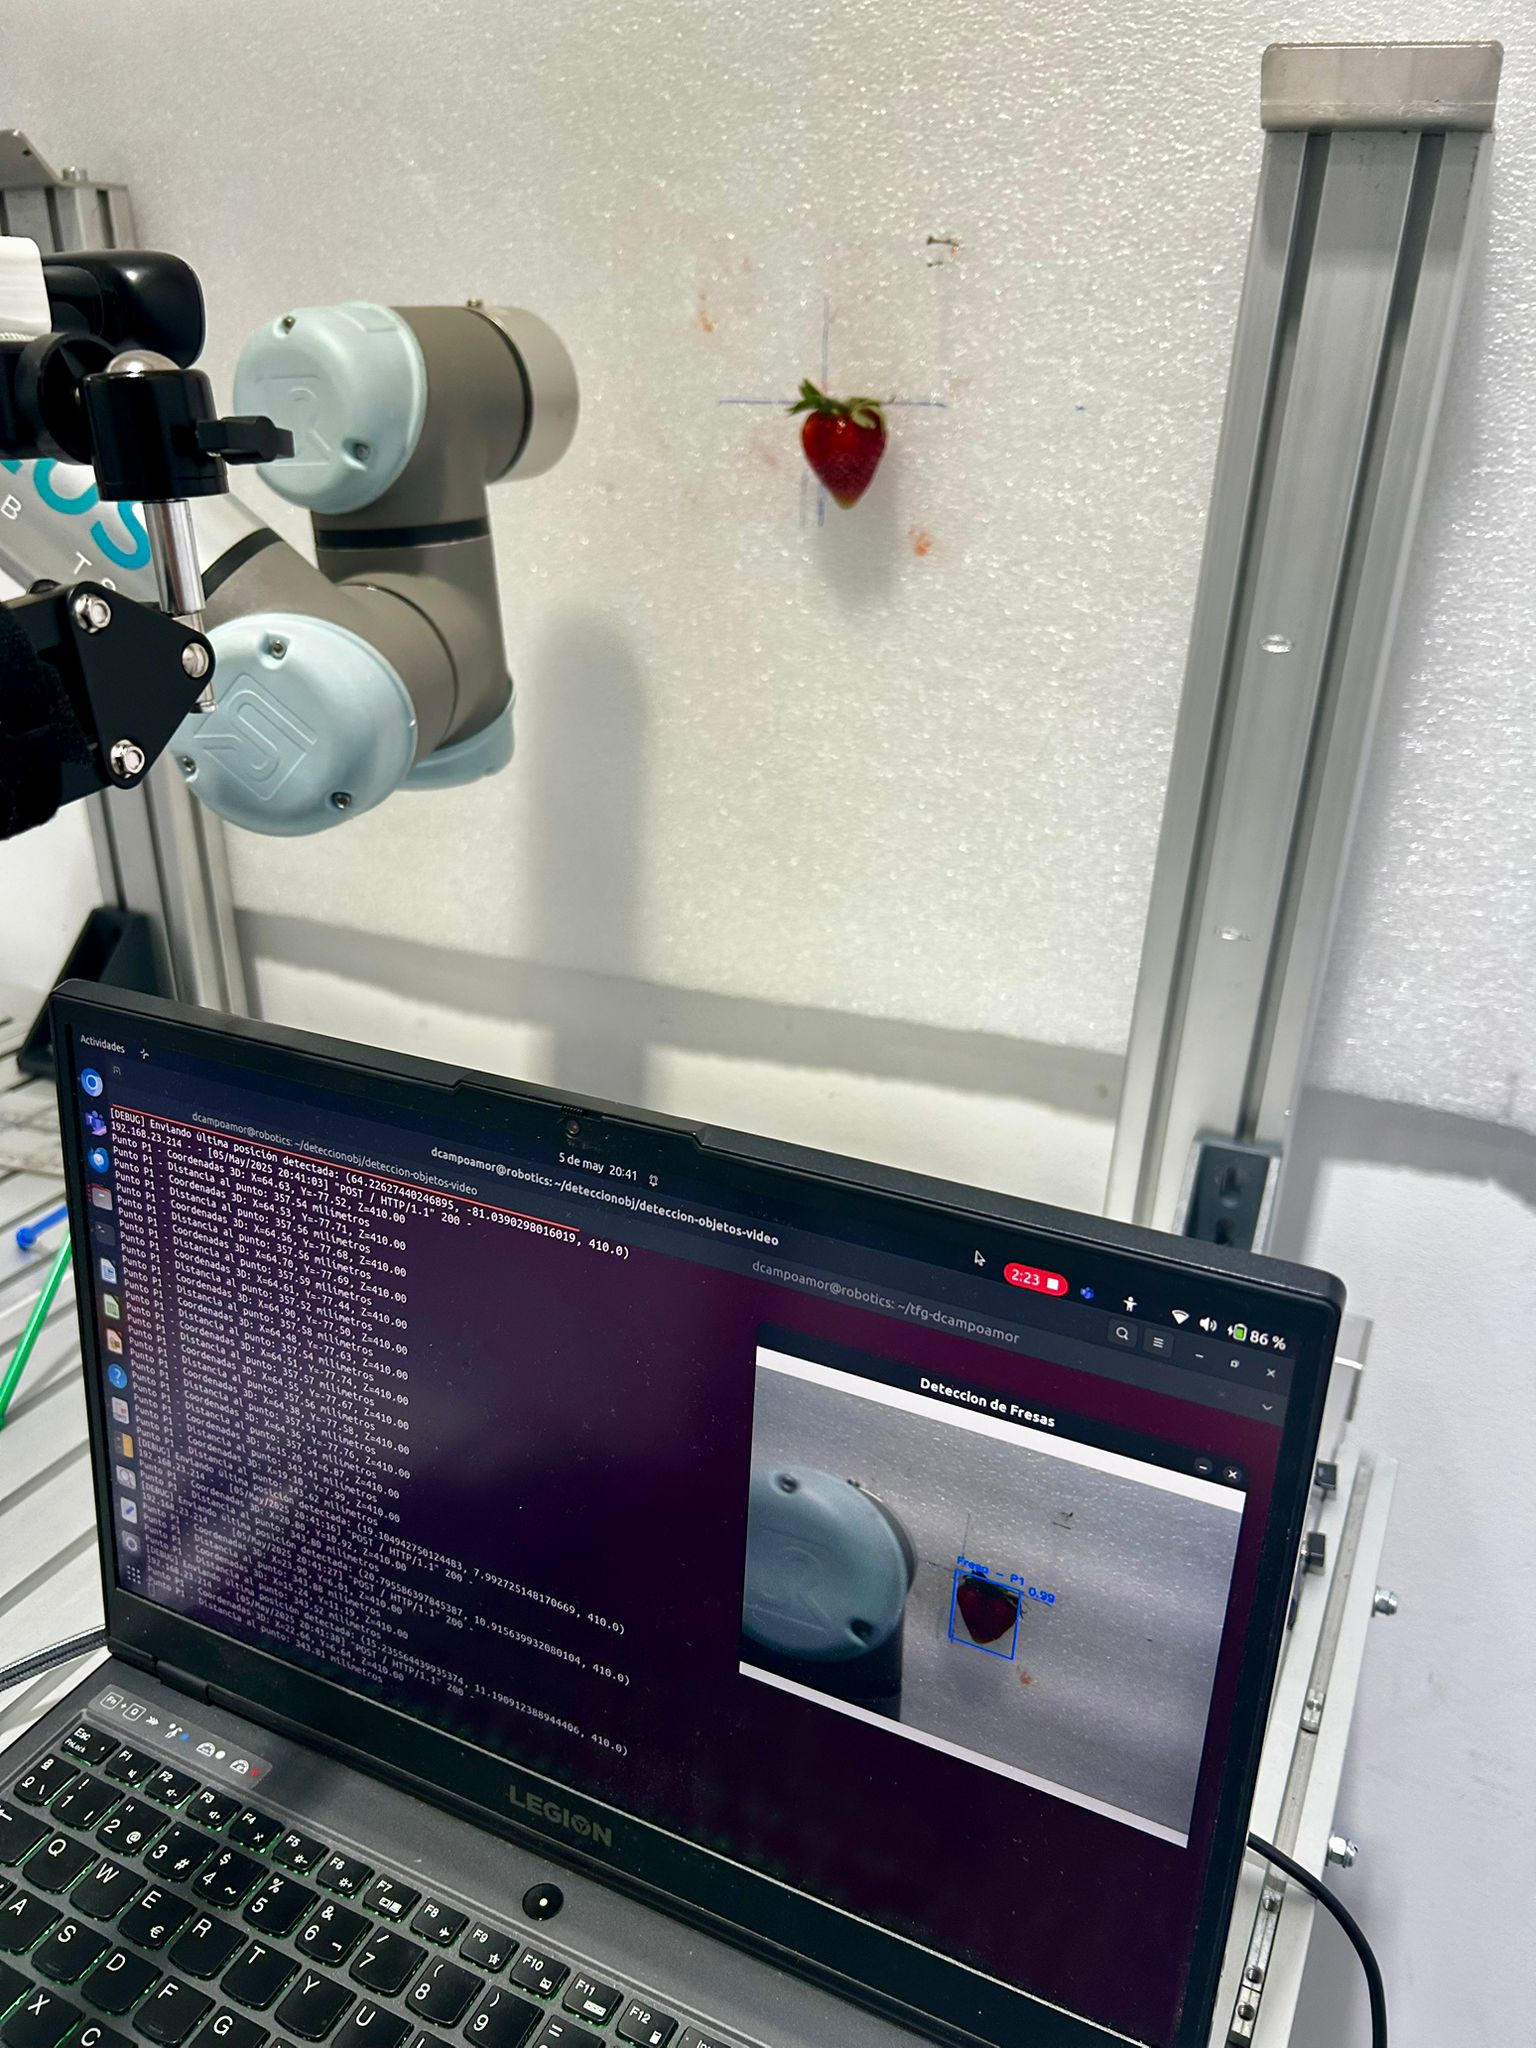
\includegraphics[width=65mm]{figs/Pruebas plano vertical deteccion simple UR5e.jpeg}}
        \hspace{1mm}
        \subfigure[Detección múltiple en el plano vertical]{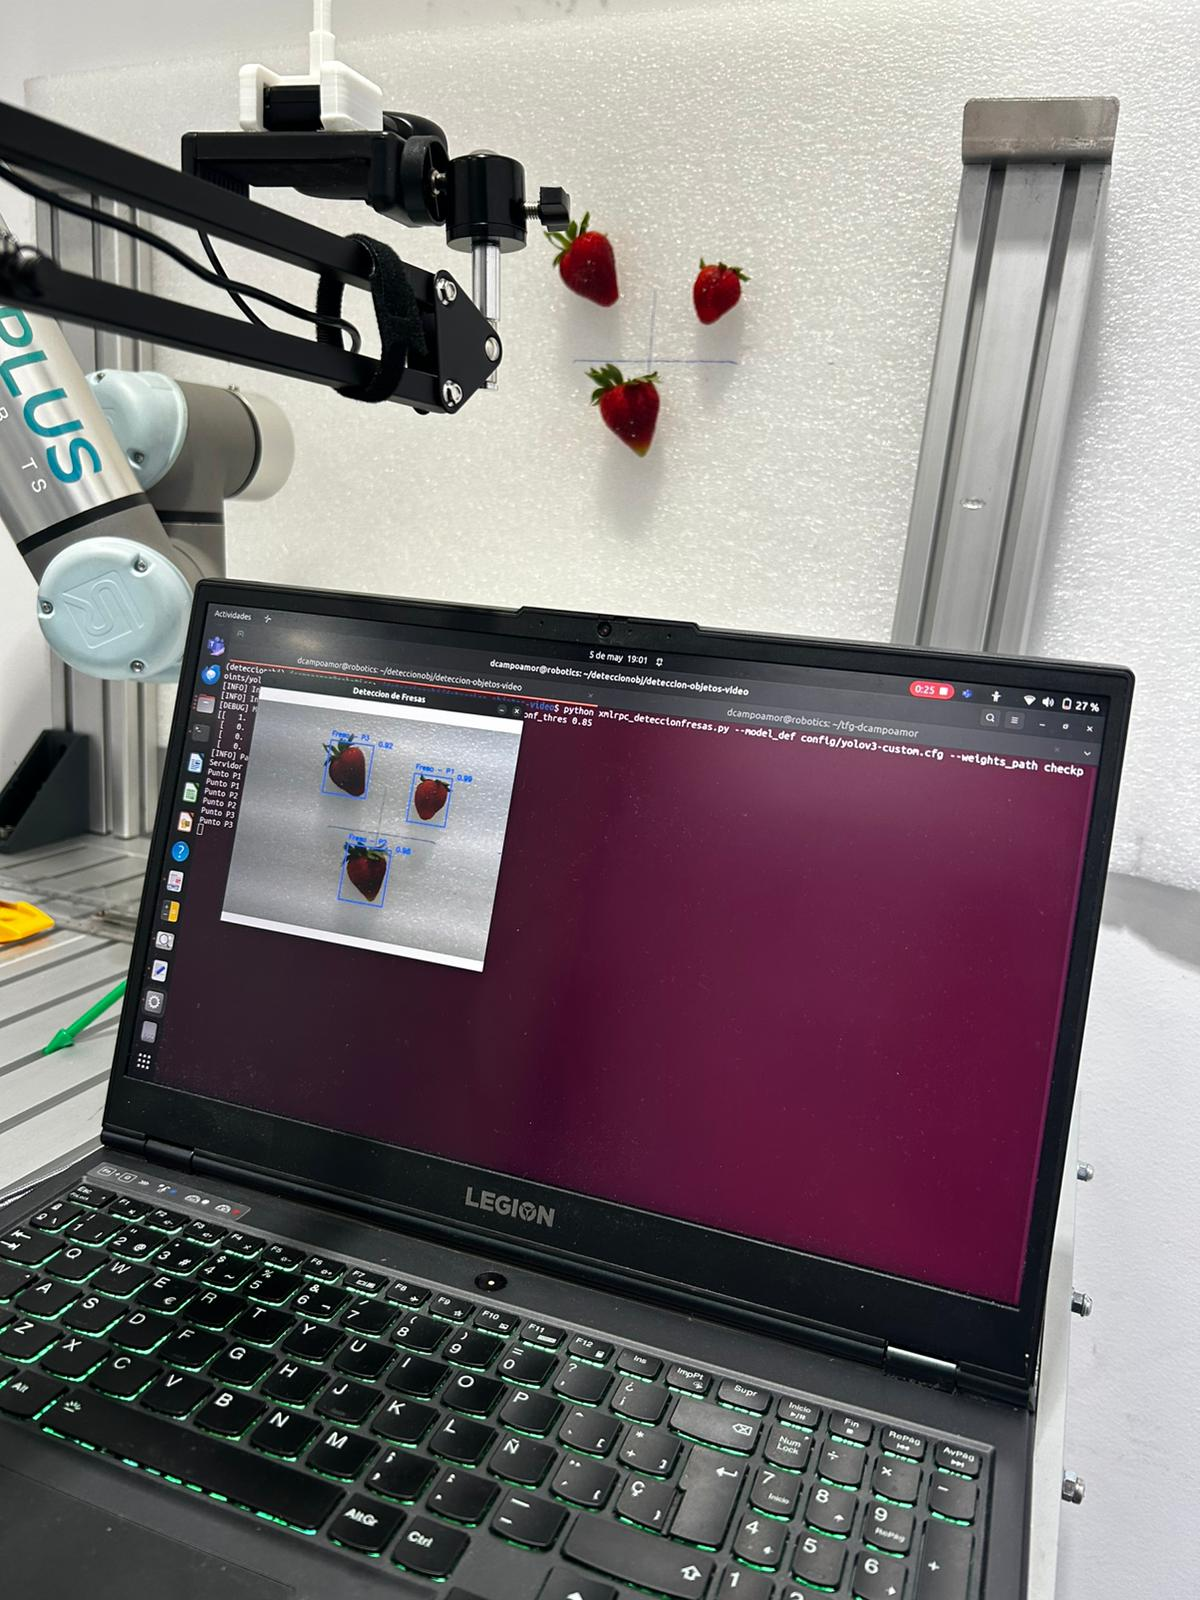
\includegraphics[width=65mm]{figs/Pruebas plano vertical deteccion multiple UR5e.jpeg}}
      \end{center}
      \caption{Disposición de las detecciones para un plano horizontal con un UR5e}
      \label{fig:UR5e_planopared}
   \end{figure}

A partir de esta base, este apartado expone el proceso completo de integración y funcionamiento coordinado de los distintos módulos que conforman la solución propuesta, siendo este el siguiente:

\begin{enumerate}
  \item La cámara captura imágenes de la escena en tiempo real.
  \item El modelo de deep learning detecta las fresas maduras y genera sus posiciones en píxeles gracias al fragmento de código del script en Python \ref{cod:dp_pixeles}.    
    \begin{code}[H]
      \begin{lstlisting}[language=Python] 
         with torch.no_grad():
              detections = model(imgTensor)
              detections = non_max_suppression(detections, opt.conf_thres, opt.nms_thres)

         positions = []
         if detections:
            for detection in detections:
                if detection is not None:
                   detection = rescale_boxes(detection, opt.img_size, frame.shape[:2])
                   for i, det in enumerate(detection):
                       if len(det) == 7:  
                           x1, y1, x2, y2, cls_conf, conf, cls_pred = det
                           box_w = x2 - x1
                           box_h = y2 - y1
                           center_x = x1 + box_w // 2
                           center_y = y1 + box_h // 2
                           color = (255, 0, 0)
                           cv2.rectangle(frame, (int(x1), int(y1)), (int(x2), int(y2)), color, 2)
                           label = f"Fresa - P{i+1}"
                           cv2.putText(frame, label, (int(x1), int(y1) - 10),
                                       cv2.FONT_HERSHEY_SIMPLEX, 0.5, color, 2)
                           confidence_text = f"{float(cls_conf):.2f}"
                           cv2.putText(frame, confidence_text, (int(x2) + 10, int(y1)),
                                       cv2.FONT_HERSHEY_SIMPLEX, 0.5, color, 2)
                           p2d = np.array([center_x, center_y])            
      \end{lstlisting}
      \caption{Fragmento del código que permite que el modelo de \textit{deep learning} detecte las fresas maduras y genere sus posiciones en píxeles}
      \label{cod:dp_pixeles}
    \end{code}

  \item Estas coordenadas se proyectan al espacio tridimensional sobre el plano vertical utilizando la función \texttt{getIntersectionZ(p2d)} (Código \ref{cod:getIntersectionZ}), que calcula la intersección del rayo proyectado con el plano Z definido por la posición de la cámara, utilizando como argumento de entrada \texttt{p2d}, es decir, las coordenadas en píxeles de la detección (Código \ref{cod:2D_a_3D}).
 
    \begin{code}[H]
      \begin{lstlisting}[language=Python] 
                           pixelOnGround3D = getIntersectionZ(p2d)
                           x_punto = float(pixelOnGround3D[0])
                           y_punto = float(pixelOnGround3D[1])
                           z_punto = float(pixelOnGround3D[2])
                           positions.append((x_punto, y_punto, z_punto)) 
      \end{lstlisting}
      \caption{Fragmento del código que realiza la retroproyección desde 2D a 3D}
      \label{cod:2D_a_3D}
    \end{code}                   
       
    \begin{code}[H]
      \begin{lstlisting}[language=Python]      
      def getIntersectionZ(p2d):
           p2d_h = np.array([p2d[0], p2d[1], 1])
           inv_K = np.linalg.inv(myCamera.k[:, :3])
           inv_RT = np.linalg.inv(myCamera.rt[:3, :3])
           p3d_h = np.dot(inv_K, p2d_h)
           p3d_h = np.dot(inv_RT, p3d_h)
           if np.abs(p3d_h[2]) > 1e-6:
               escala = -myCamera.position[2] / p3d_h[2]
               p3d_h *= escala
           return np.array(p3d_h)
      \end{lstlisting}
      \caption{Función \texttt{getIntersecionZ()}}
      \label{cod:getIntersectionZ}
    \end{code}                                    
                           
  \item El servidor XML-RPC se crea en la dirección IP y puerto especificado, se transmiten las coordenadas al robot a través de la función \texttt{get\_next\_pose()}, y lanza en un hilo independiente que queda a la espera de nuevas peticiones (Código \ref{cod:get_next_pose}).
  
    \begin{code}[H]
      \begin{lstlisting}[language=Python] 
      # Conexion con el robot usando XML-RPC
      server = SimpleXMLRPCServer(("192.168.23.107", 50000))
      server.RequestHandlerClass.protocol_version = "HTTP/1.1"
      print("Servidor XML-RPC corriendo en el puerto 50000...")
      
      def get_next_pose():
          if detected_points:
              pose = detected_points[-1]
              print(f"[DEBUG] Enviando ultima posicion detectada: {pose}")
              return [pose[0], pose[1], pose[2], 0, 0, 0]
          else:
              print(f"[DEBUG] No se detectaron puntos, enviando posicion de inicio")
              return [0, 0, 0, 0, 0, 0]

      server.register_function(get_next_pose, "get_next_pose")
      import threading
      server_thread = threading.Thread(target=server.serve_forever)
      server_thread.daemon = True
      server_thread.start()
      \end{lstlisting}
      \caption{Envío de la última posición tridimensional detectada al robot mediante XML-RPC}
      \label{cod:get_next_pose}
    \end{code}          
  
  \item El robot interpreta la posición, calcula una trayectoria y actúa sobre la fruta detectada (Figura \ref{fig:Config_comunicación_UR}).
    \begin{figure}[H]
      \begin{center}
        \subcapcentertrue
        \subfigure[Configuración de la comunicación XMLRPC en el robot]{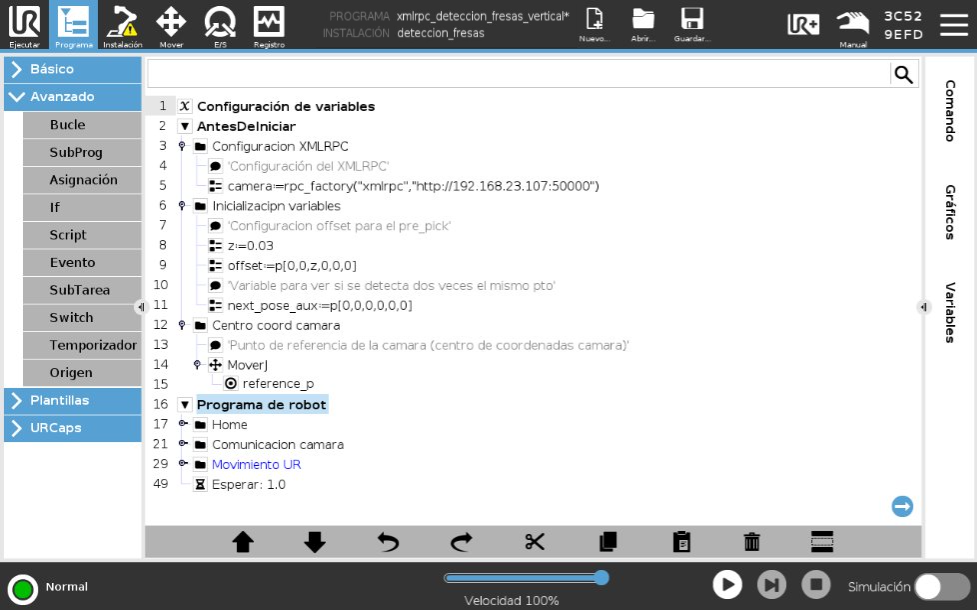
\includegraphics[width=155mm]{figs/Antes de Iniciar_XMLRPC.png}}
        \hspace{4mm}
        \subfigure[Instrucciones de movimiento del robot según la casuística]{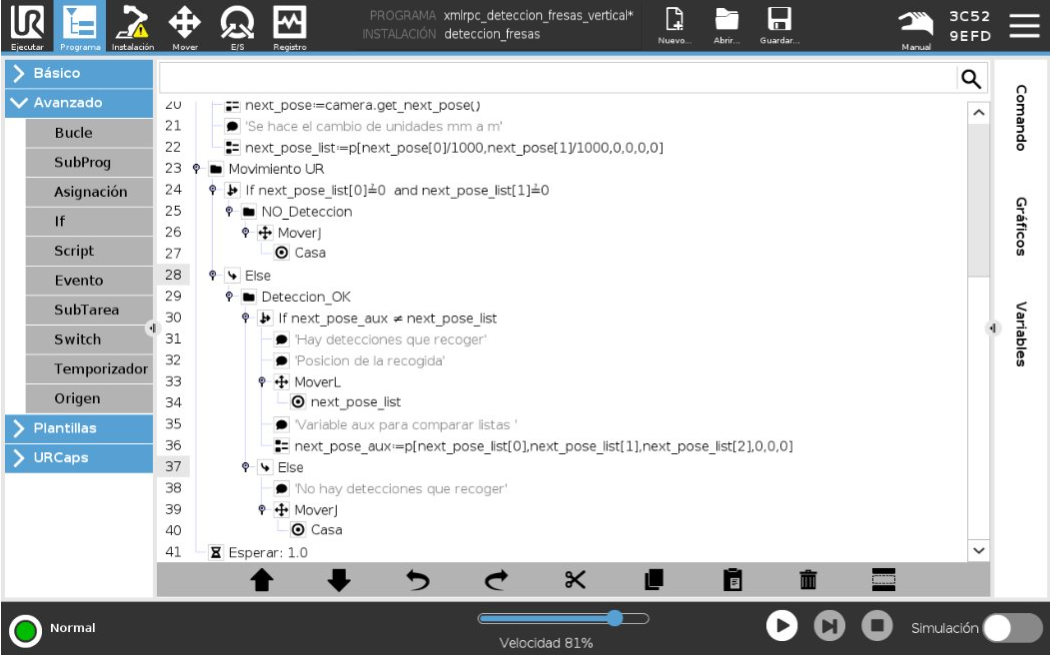
\includegraphics[width=155mm]{figs/Movimiento UR.png}}
      \end{center}
      \caption{Ajustes de comunicación XMLRPC en el robot y ejecución de movimientos definidos en el programa}
      \label{fig:Config_comunicación_UR}
    \end{figure}
 
\end{enumerate}


Esta arquitectura permite un sistema modular, robusto y fácilmente escalable a escenarios reales más complejos, sentando las bases para su posible aplicación futura en entornos agrícolas reales o semiautomatizados. Para hacer funcionar el sistema completo y conseguir una correcta integración entre el sistema de visión y el brazo robótico UR, deben seguirse los siguientes pasos de forma ordenada.

\begin{enumerate}
  \item Conexión de red: Es fundamental asegurar que, tanto el robot como el ordenador que ejecuta el sistema de visión, están conectados a la misma red local y que ambos dispositivos pertenezcan a la misma subred, recomendándose el uso de cables ethernet para una mayor estabilidad. Por este motivo, es necesario comprobar que hay conectividad entre ambos dispositivos (por ejemplo, mediante el uso del comando \texttt{ping} a la IP del robot desde el ordenador), ya que la comunicación se establece a través del protocolo XML-RPC sobre una dirección IP y puerto determinados.
    
      \begin{figure} [H]
        \begin{center}
          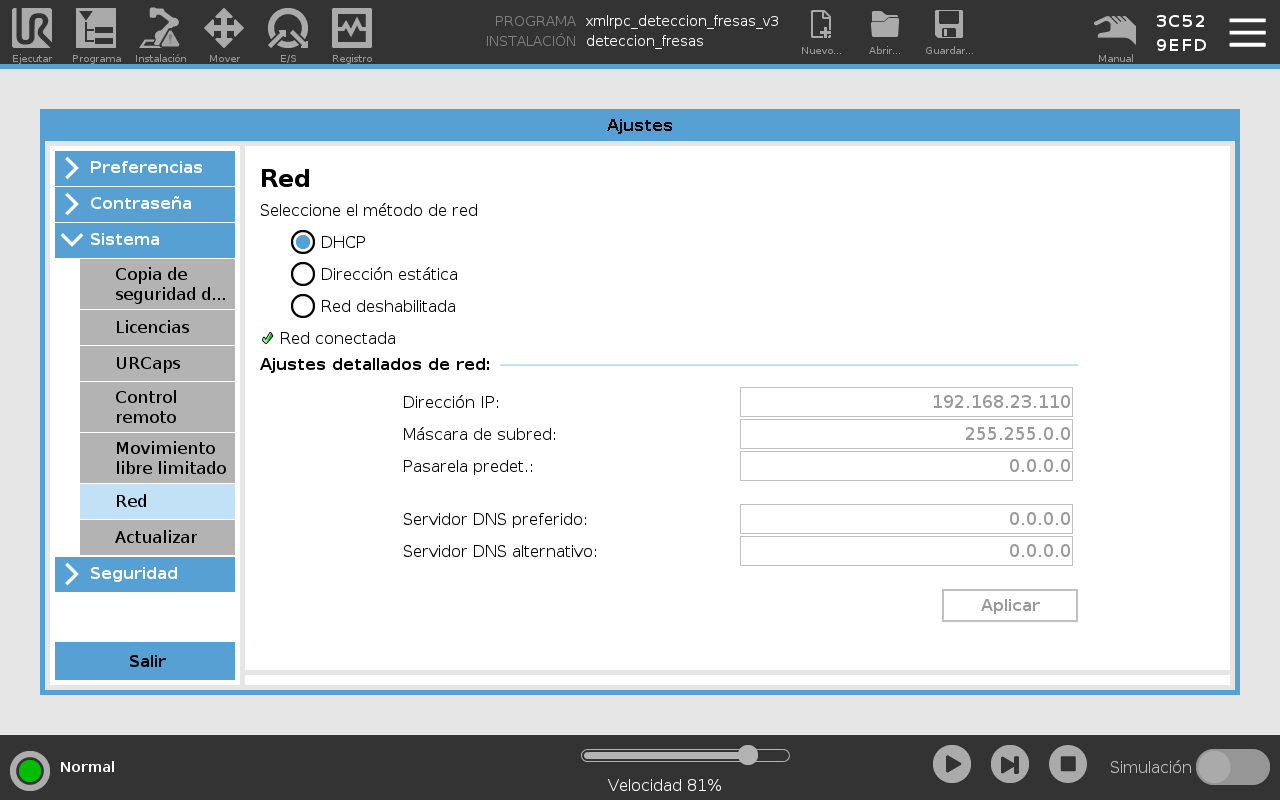
\includegraphics[width=155mm]{figs/Ajustes de Red UR.png}
        \end{center}
        \caption{Ajustes de red en el robot}
        \label{fig:ajustes_red_UR}
      \end{figure} 
  
  \item Definición de la Instalación del robot: Si el robot lleva instalado un efector final, como una garra o un actuador, es importante configurar correctamente la carga útil, el peso y el centro de gravedad en el software del UR, ya que esto garantiza un funcionamiento seguro y preciso, ajustando los parámetros de control de movimiento y compensación de la cinemática.
  
    \begin{figure}[H]
      \begin{center}
        \subcapcentertrue
        \subfigure[Configuración del Punto Central de la Herramienta (PCH)]{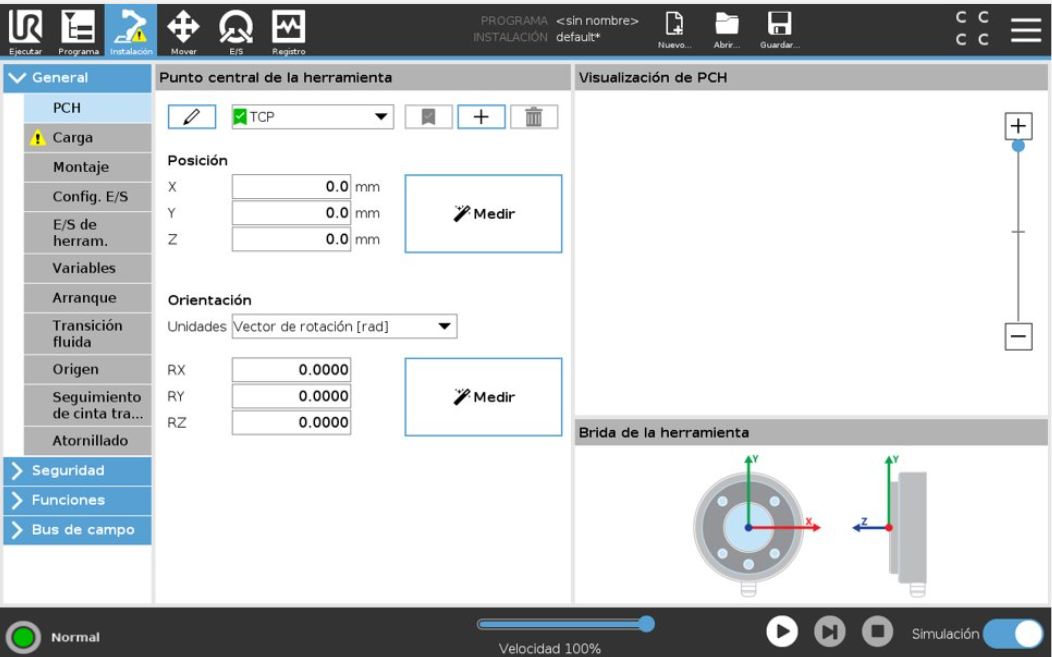
\includegraphics[width=155mm]{figs/Config_PCH.png}}
        \hspace{4mm}
        \subfigure[Configuración de la carga]{\includegraphics[width=155mm]{figs/config_Carga.png}}
      \end{center}
      \caption{Definición de la Instalación del efector final en el robot}
      \label{fig:Config_UR}
    \end{figure}
    
  \pagebreak
  \item Creación del plano de trabajo: A continuación, se debe definir el plano de trabajo sobre el que se va a operar, en este caso un plano vertical, como se detalló en la Sección \ref{sec:HS_vertical}. 
  
  \item Lanzamiento del sistema de comunicación: En este punto, se debe ejecutar el script en Python mediante la línea de comando que se muestra a continuación. Para este caso, es el programa \textit{xmlrpc\_deteccionfresas.py}\footnote{\url{https://github.com/RoboticsURJC/tfg-dcampoamor/blob/main/src/robot/xmlrpc_deteccionfresas.py}} el que ejerce de servidor, y tiene que ejecutarse desde la terminal del ordenador para poder ejecutar posteriormente mediante el botón de \textit{play} de la interfaz del robot, el programa \textit{xmlrpc\_deteccion\_fresas\_vertical.urp}\footnote{\url{https://github.com/RoboticsURJC/tfg-dcampoamor/blob/main/src/robot/xmlrpc_deteccion_fresas_vertical.urp}}, que realiza la solicitud de datos al servidor remoto a través del protocolo XML-RPC, una vez que el servidor esté en marcha.
  
\small
\begin{verbatim}
python xmlrpc_deteccionfresas.py --model_def config/yolov3-custom.cfg 
--weights_path checkpoints/yolov3_ckpt_99.pth 
--class_path data/custom/classes.names --conf_thres 0.85 
\end{verbatim}  
\normalsize
    
    %\begin{figure} [H]
    %   \begin{center}
    %      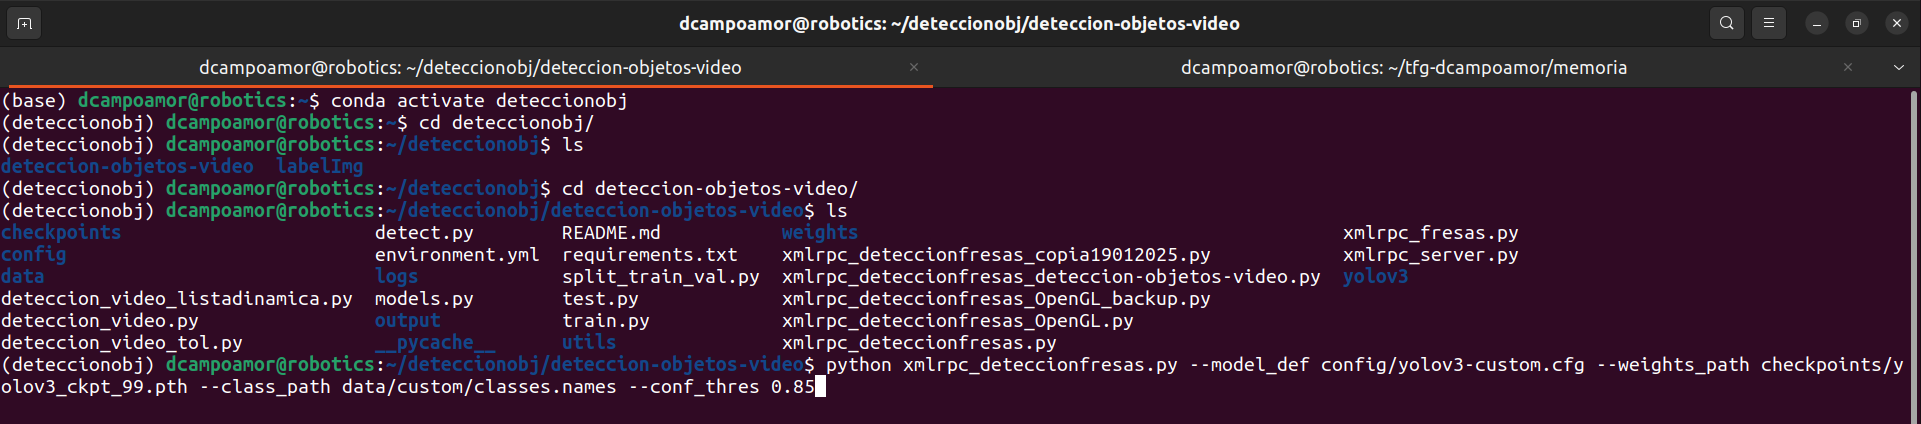
\includegraphics[width=135mm]{figs/Ejecutar_Programa_Python.png}
    %    \end{center}
    %    \caption{Lanzamiento del servidor mediante el programa en Python en la terminal del ordenador}
    %    \label{fig:ejecucion_python}
    %\end{figure} 

  \item Ejecución: Una vez en marcha tanto el programa en el ordenador como en el robot, el sistema detectará automáticamente las fresas presentes en la escena, calculará sus coordenadas tridimensionales y las enviará al robot, que ejecutará el movimiento correspondiente según el programa \textit{xmlrpc\_deteccion\_fresas\_vertical.urp}\footnote{\url{https://github.com/RoboticsURJC/tfg-dcampoamor/blob/main/src/robot/xmlrpc_deteccion_fresas_vertical.urp}}, para acercarse a la fresa y situarse encima de esta para una futura recolección.
      
%    \begin{figure}[H]
%      \begin{center}
%        \subcapcentertrue
%        \subfigure[Ejecución del programa en Python en la terminal del ordenador]{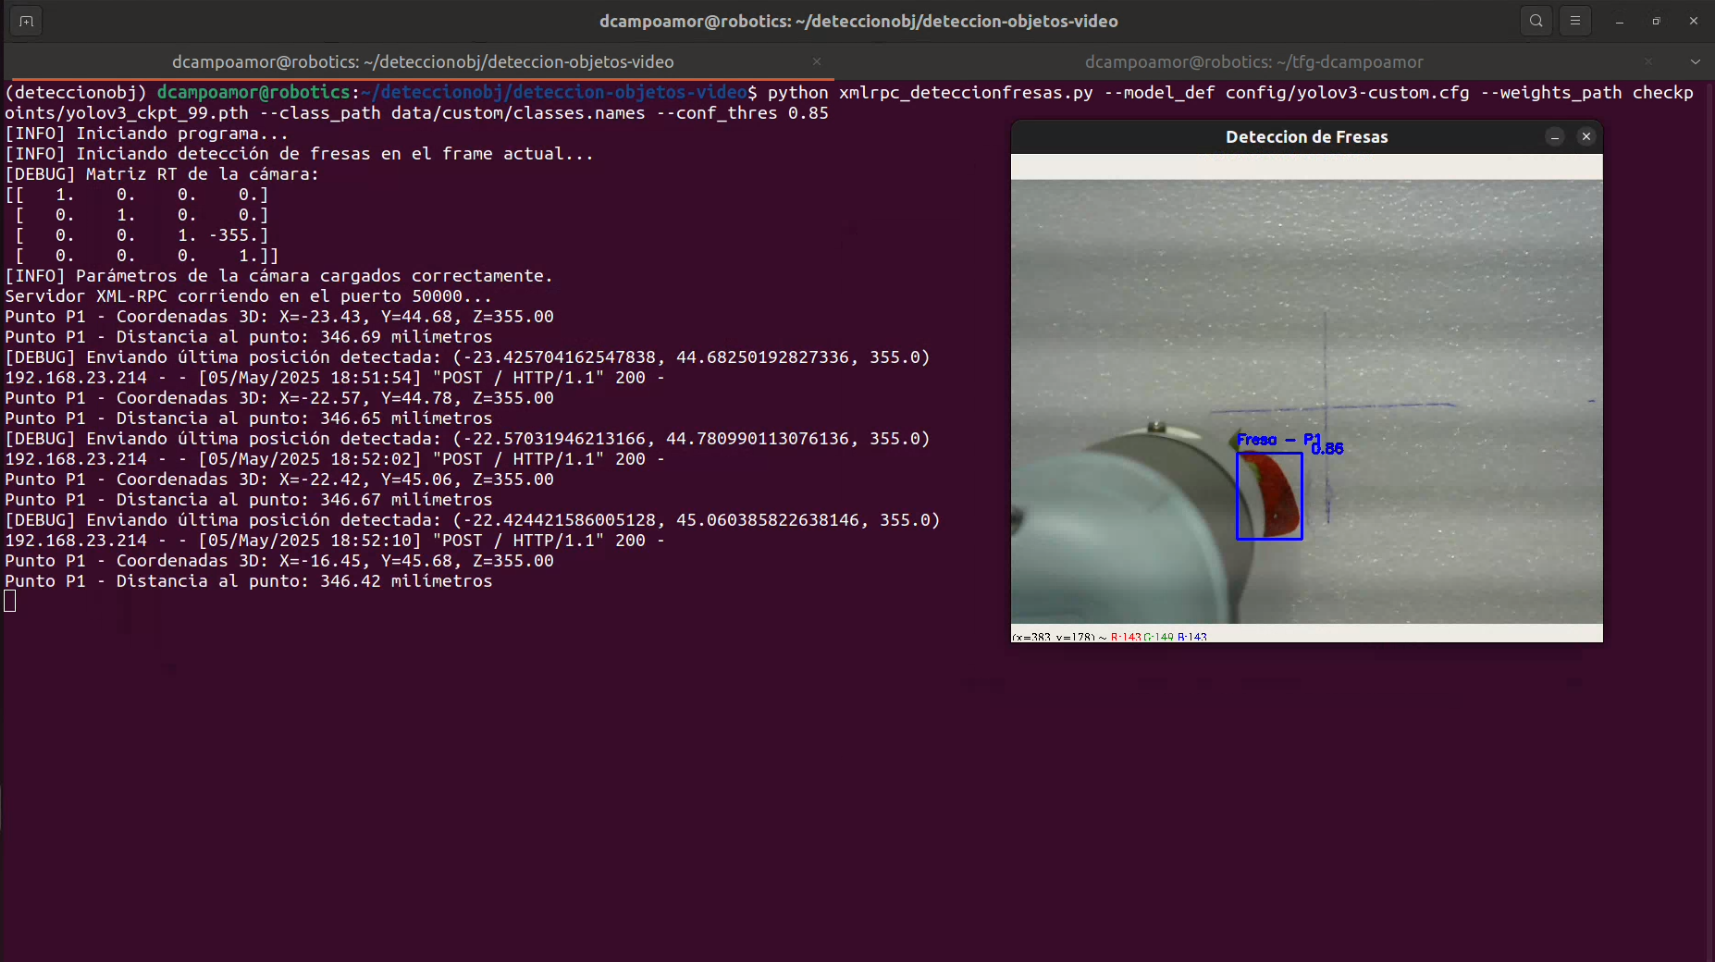
\includegraphics[width=78mm]{figs/POV Camara Pruebas plano vetical deteccion simple UR5e}}
%        \hspace{4mm}
%        \subfigure[Ejecución del programa de robot]{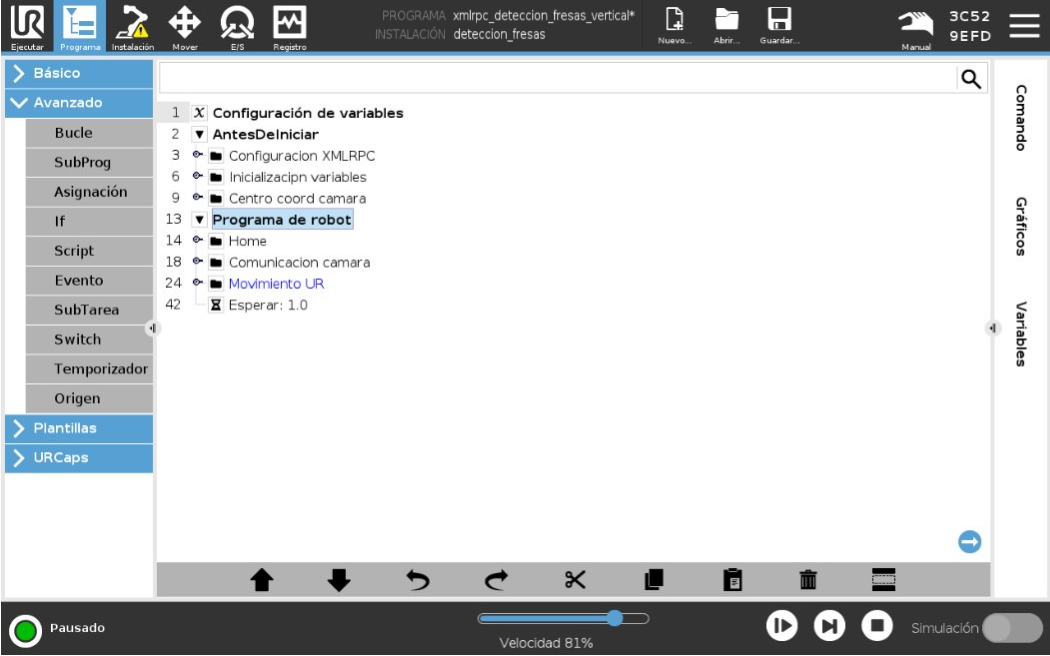
\includegraphics[width=70mm]{figs/Carpetas del Programa UR.png}}
%      \end{center}
%      \caption{Ejecución de los programas de manera simultánea}
%      \label{fig:Ejecucion_programas}
%    \end{figure}
\end{enumerate}

Para completar la evaluación del prototipo, a pesar de que no se llegó a implementar la acción de cierre o agarre de la pinza dentro del flujo automatizado del sistema, se realizaron pruebas complementarias utilizando una pinza industrial acoplada al robot en el programa de robot \textit{xmlrpc\_deteccion\_fresas\_vertical\_pinza.urp}\footnote{\url{https://github.com/RoboticsURJC/tfg-dcampoamor/blob/main/src/robot/xmlrpc_deteccion_fresas_vertical_pinza.urp}} (Figura \ref{fig:Programa_UR_pinza}) con el objetivo de verificar la compatibilidad y robustez del programa desarrollado. Estas pruebas permitieron demostrar que el sistema era plenamente funcional y adaptable, y que se podía integrar sin inconvenientes cualquier herramienta de agarre que fuera adecuada para el manejo de fresas, dada su delicadeza. De este modo, se confirma que el sistema de detección, proyección y comunicación con el robot puede extenderse fácilmente para incluir un actuador final destinado a la recolección efectiva del fruto en un entorno real (Figura \ref{fig:UR5e_planopared_garra}).

   \begin{figure}[H]
      \begin{center}
        \subcapcentertrue
        \subfigure{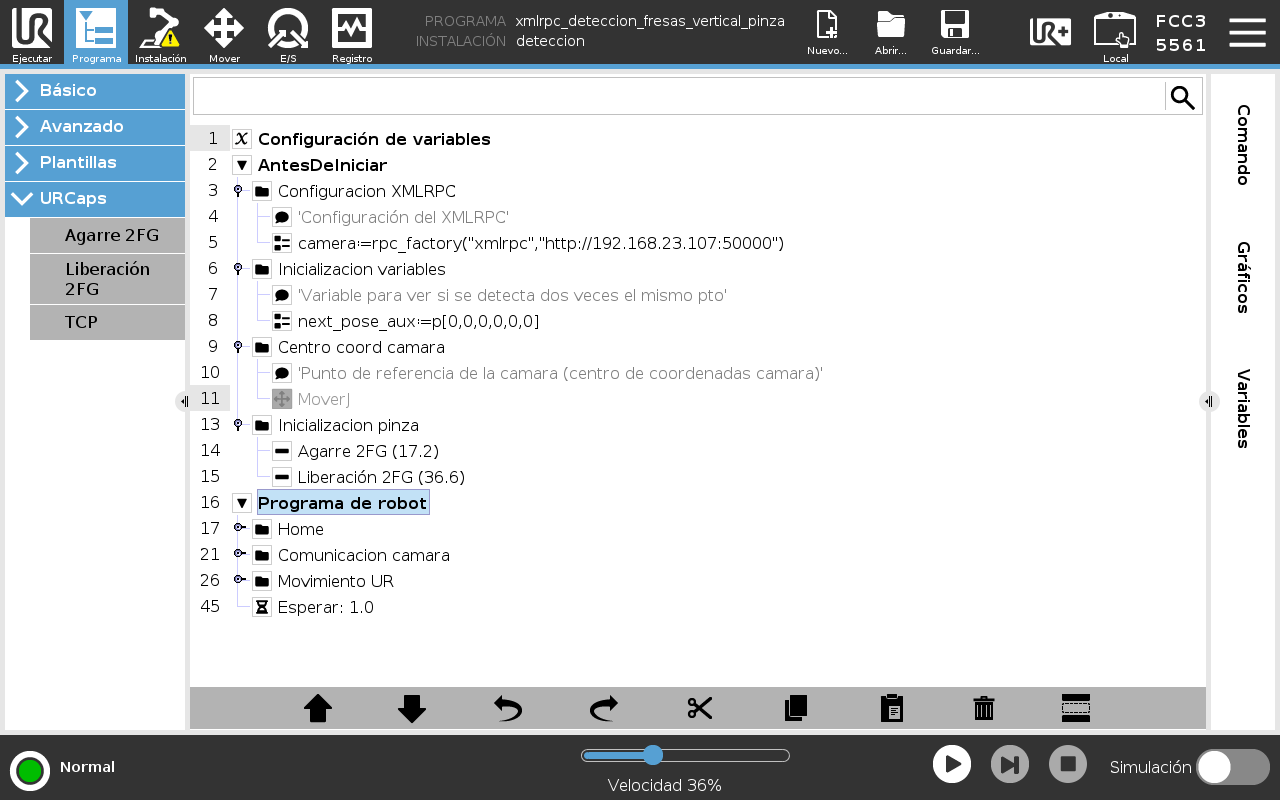
\includegraphics[width=155mm]{figs/Antes de Iniciar Programa UR Pinza.png}}
        \hspace{1mm}
        \subfigure{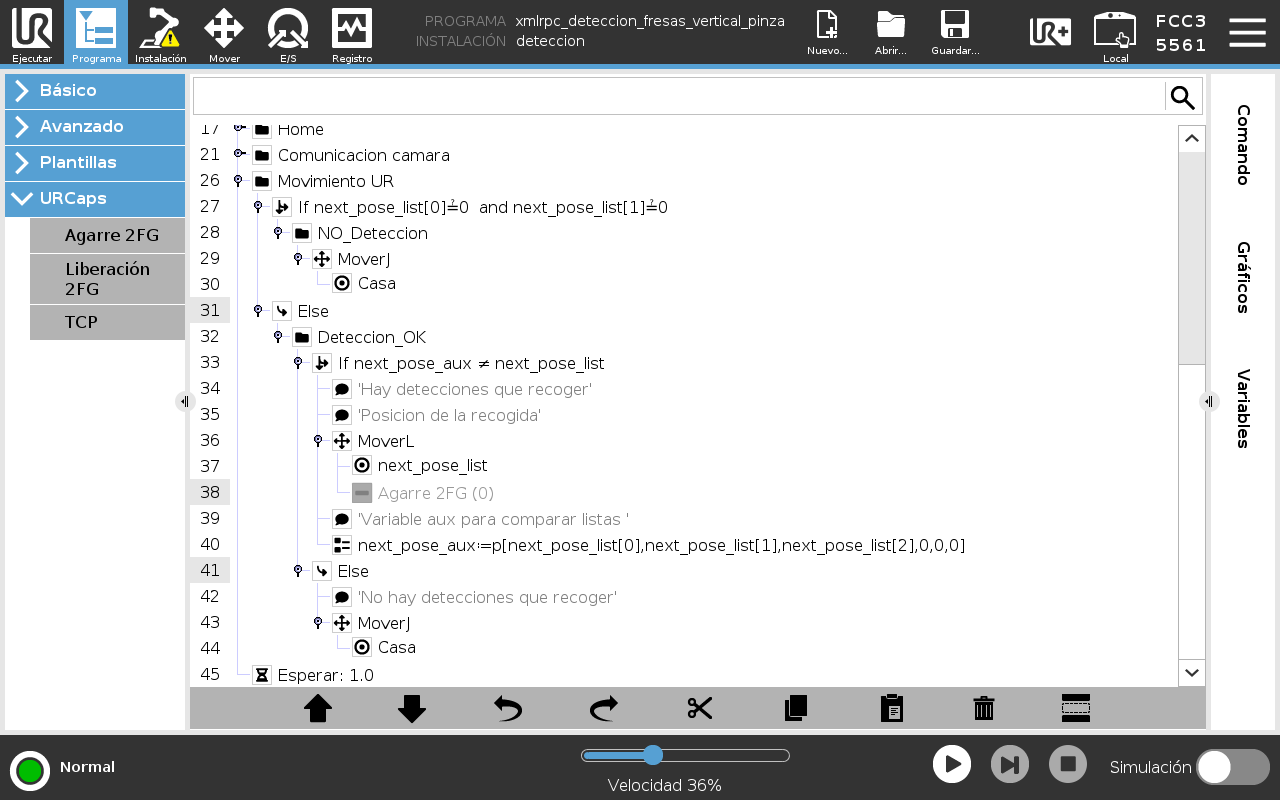
\includegraphics[width=155mm]{figs/Movimiento UR Programa UR Pinza.png}}
      \end{center}
      \caption{Programa \textit{xmlrpc\_deteccion\_fresas\_vertical\_pinza.urp} para uso del sistema con efector final}
      \label{fig:Programa_UR_pinza}
   \end{figure}
   
   
   \begin{figure}[H]
      \begin{center}
        \subcapcentertrue
        \subfigure{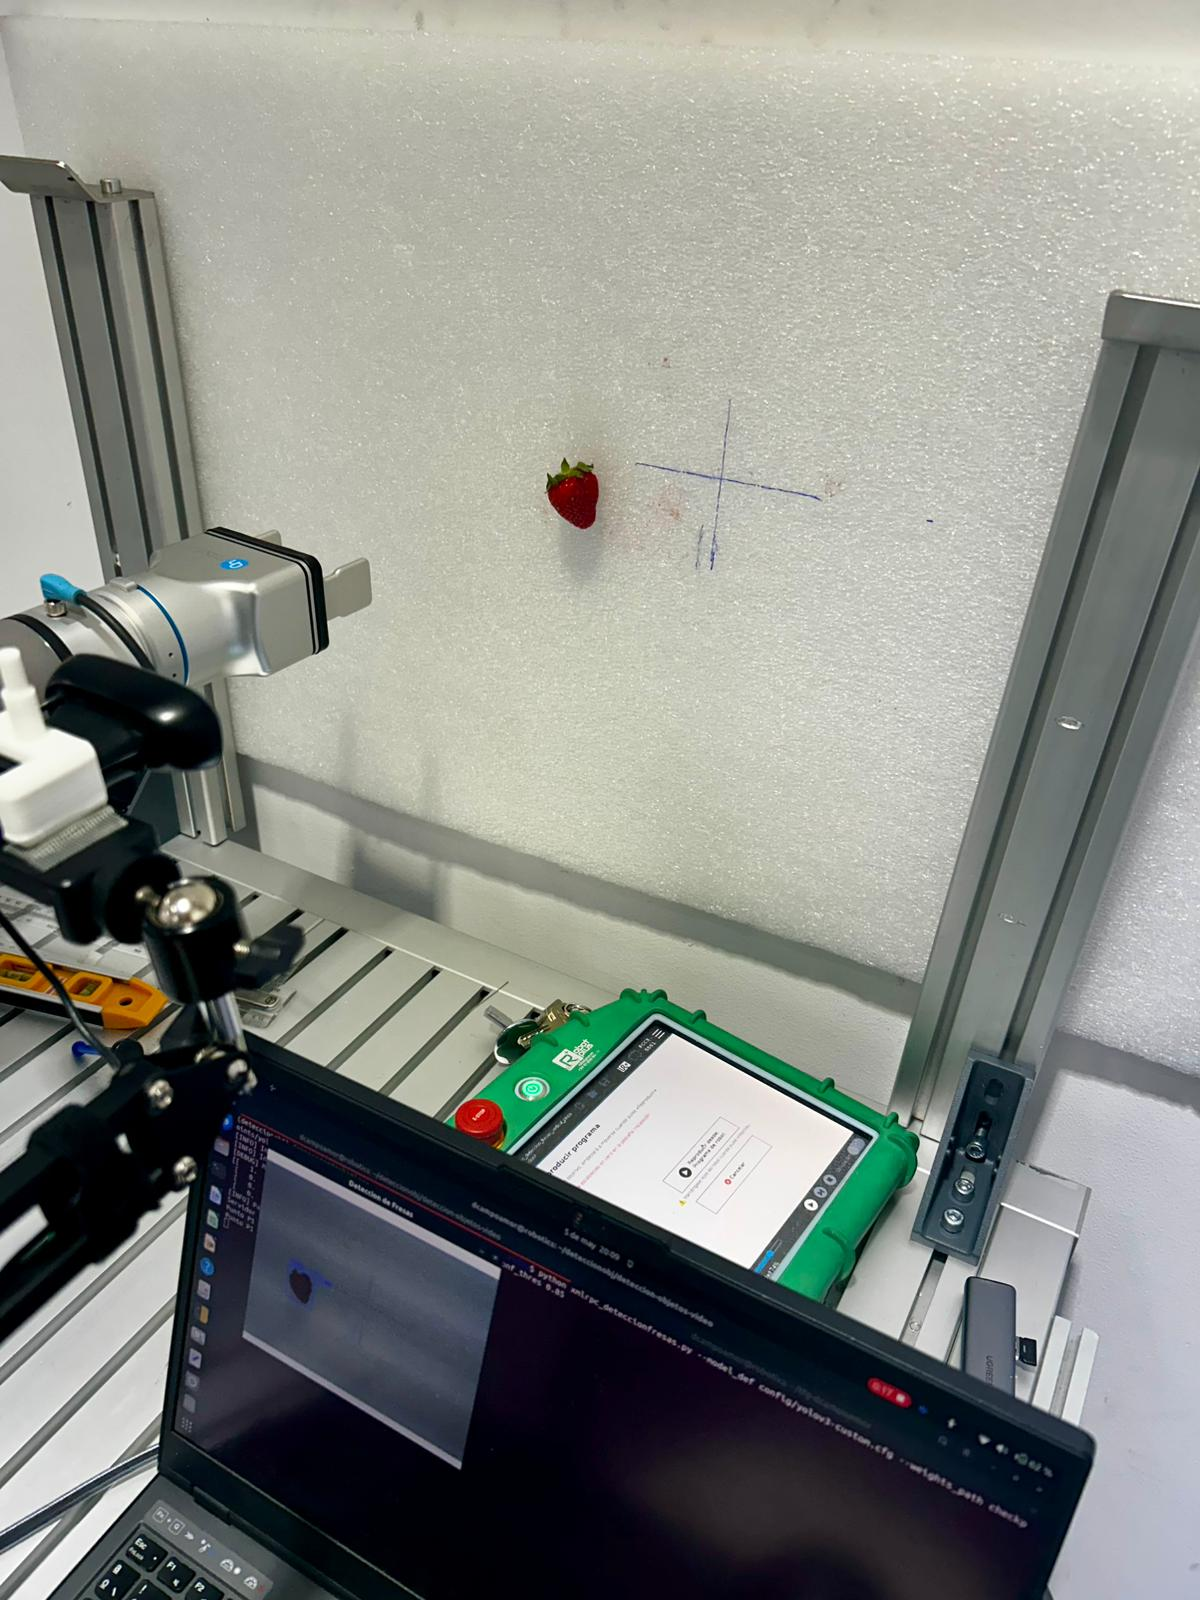
\includegraphics[width=69mm]{figs/Pruebas plano vertical deteccion simple garra UR5e.jpeg}}
        \hspace{1mm}
        \subfigure{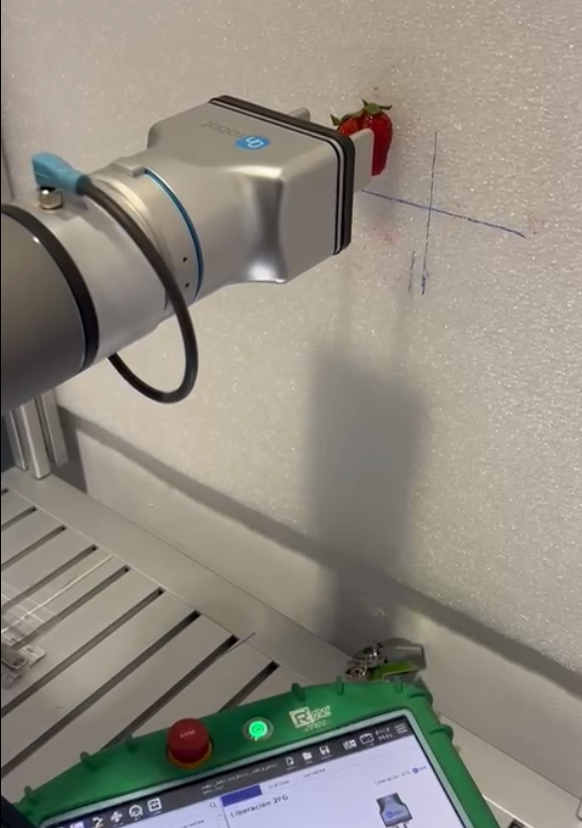
\includegraphics[width=65mm]{figs/Pruebas plano vertical deteccion simple garra UR5e_2.png}}
      \end{center}
      \caption{Pruebas en el plano vertical de detección con garra integrada}
      \label{fig:UR5e_planopared_garra}
   \end{figure}

\vspace{5mm}

En este capítulo, se ha descrito en detalle el sistema desarrollado, incluyendo los fundamentos técnicos, las herramientas de visión artificial empleadas, y el proceso de integración con el robot colaborativo UR, siendo un sistema diseñado con el objetivo de ser modular, reproducible y eficaz en tareas de detección y recolección de frutos maduros en entornos controlados. En el Anexo \ref{cap:capitulo8}, se presentan los experimentos realizados, donde se detallan las diferentes pruebas llevadas a cabo, los ajustes realizados durante el desarrollo y los resultados obtenidos hasta alcanzar el estado funcional final del proyecto. De igual manera, puede encontrarse mayor documentación gráfica en el repositorio público de GitHub\footnote{\url{https://github.com/RoboticsURJC/tfg-dcampoamor}} dedicado al proyecto; como por ejemplo, vídeos del funcionamiento del sistema conjunto, tanto sin efector final, como el vídeo \textit{Pruebas plano vertical detección múltiple UR5e.mp4}\footnote{\url{https://github.com/RoboticsURJC/tfg-dcampoamor/blob/main/img/code/UR/Pruebas\%20plano\%20vertical\%20deteccion\%20multiple\%20UR5e.mp4}}, como vídeos del sistema conjunto con efector final, tal cual se muestra en \textit{Pruebas plano vertical detección simple garra UR5e.mp4}\footnote{\url{https://github.com/RoboticsURJC/tfg-dcampoamor/blob/main/img/code/UR/Pruebas\%20plano\%20vertical\%20deteccion\%20simple\%20garra\%20UR5e.mp4}}, entre otros.

















